\documentclass[10pt,a4paper]{article}
\usepackage[a4paper, top=2cm, bottom=1.5cm, left=1.5cm, right=1.5cm]{geometry} % Задать размеры полей.
\usepackage[warn]{mathtext} % Русские символы в формулах. Нужно писать до пакета babel. Указывает, что в формулах используются символы кириллицы, которые по умолчанию печатаются прямым шрифтом.
\usepackage[T2A]{fontenc}
\usepackage[utf8]{inputenc}
\usepackage[russian]{babel}
\usepackage{amsmath}
\usepackage{amssymb}
\usepackage{graphicx}
\usepackage{floatrow}
\usepackage{booktabs}
\usepackage{wrapfig}
\usepackage{lipsum}
\usepackage{mathtools}
\usepackage{verbatim}
%\usepackage{subcaption}
\usepackage{fancyhdr}
\usepackage{multicol}
\usepackage{xcolor}

%multi-column
%\multicolumn{number cols}{align}{text} % align: l,c,r

%multi-row
\usepackage{multirow}

\newcommand{\cell}[2]{
	\begin{tabular}{c}$#1$ \\ $#2$\end{tabular}}

\newcommand{\cellv}[3]{
	\begin{tabular}{c}$#1$ \\ $#2$ \\ $#3$\end{tabular}}

\newcommand{\figref}[1]{(См. рис. \ref{#1})}
\newcommand{\secref}[1]{(См. раздел. \ref{#1})}

\newcommand{\adecay}[2]{\xrightarrow[\cell{#1}{#2}]{\alpha}}
\newcommand{\bpdecay}[2]{\xrightarrow[\cell{#1}{#2}]{\beta^+}}
\newcommand{\bmdecay}[2]{\xrightarrow[\cell{#1}{#2}]{\beta^-}}

\newcommand{\avdecay}[3]{\xrightarrow[\cellv{#1}{#2}{#3}]{\alpha}}
\newcommand{\bpvdecay}[3]{\xrightarrow[\cellv{#1}{#2}{#3}]{\beta^+}}
\newcommand{\bmvdecay}[3]{\xrightarrow[\cellv{#1}{#2}{#3}]{\beta^-}}

\newcommand{\e}[1]{\text{$\cdot10^{#1}$}}

% Единицы измерения.
% Использование:
% В формуле, когда нужен пробел после числа, нужно ввести просто название команды.
% Пример:
%     $1.5 \pm 0.1 \sec$
%     Результат будет примерно следующий: 1.5+-0.1 c
% Если пробел перед единицами измерения не нужен, то после названия команды нужно ввести []. 
% Пример:
%     $1.5 \pm 0.1 \sec[]$
%     Результат будет примерно следующий: 1.5+-0.1c
\newcommand{\atm}[1][\;]{#1 атм.}
\newcommand{\mmhg}[1][\;]{#1 мм рт.ст.}
\newcommand{\Bk}[1][\;]{#1 Бк}
\newcommand{\MeV}[1][\;]{#1 МэВ}
\newcommand{\keV}[1][\;]{#1 кэВ}
\newcommand{\eV}[1][\;]{#1 эВ}
\newcommand{\msec}[1][\;]{#1 мс}
\renewcommand{\sec}[1][\;]{#1 с}
\renewcommand{\min}[1][\;]{#1 м}
\newcommand{\hour}[1][\;]{#1 ч}
\renewcommand{\day}[1][\;]{#1 д}
\renewcommand{\year}[1][\;]{#1 л}

\newcommand{\stable}[1][\;]{#1 (ст.)}

\newcommand{\elem}[3]{{}^{#2}_{#3}\text{#1}}
\newcommand{\Ra}{\elem{Ra}{226}{88}}
\newcommand{\Pu}{\elem{Pu}{239}{94}}
\newcommand{\Po}{\elem{Po}{210}{84}}
\newcommand{\Ua}{\elem{U}{238}{92}}
\newcommand{\Ub}{\elem{U}{234}{92}}
\newcommand{\Th}{\elem{Th}{230}{90}}
\newcommand{\Am}{\elem{Am}{241}{95}}

\pagestyle{fancy}
\fancyhead{}
\fancyhead[L]{\small Маслов А.С., Дедков Д.А., Измерение спектров $\alpha$-излучения ядрами $\Ra$, $\Po$, $\Pu$, $\Ua$, и смеси ($\Th$ и $\Am$) с помощью полупроводникового детектора. МФТИ, 2023 г.}
\fancyhead[R]{}
\fancyfoot[C]{\thepage}

\renewcommand{\cot}{\text{ctg}}

\author{\normalsize Маслов Артём, Дедков Денис \\
	\normalsize группа Б01-108а \\
	\normalsize 11.09.2023}
\date{}

\usepackage{float}
\restylefloat{table}
\title{
	\Large Измерение спектров $\alpha$-излучения ядер $\Ra$, $\Po$, $\Pu$, $\Ua$ и смеси ($\Th$ и $\Am$) с помощью полупроводникового детектора. \\ 
}

\addto\captionsrussian{\def\refname{Литература}}

\begin{document}
\maketitle
\begin{multicols}{2}
	
	\subsection*{Аннотация}
	
	В работе измеряются спектры $\alpha$-излучения ядер $\Ra$, $\Po$, $\Pu$, $\Ua$ и смеси ($\Th$ и $\Am$) с помощью полупроводникового детектора. Исследуются последовательные $\alpha$-распады указанных ядер. Проверяется закон Гейгера-Нэттола для ядер $\Ra$ на основе табличных значений.
	
	\textbf{Ключевые слова:} $\alpha$-распад, закон Гейгера-Нэттола.
	
	\subsection*{Введение}
	\textit{Альфа-распадом} называется самопроизвольный процесс испускания ядрами альфа-частиц:
	$$
	\elem{X}{A}{Z} \rightarrow \elem{$X'$}{A-4}{Z-2} + \elem{He}{4}{2}
	$$
	Периодом полураспада $T_{1/2}$ называется время в течение которого количество радиоактивных атомов убывает в 2 раза. Если $N_0$ -- начальное количество радиоактивных атомов, то количество атомов $N(t)$ в последующие моменты времени определяется \textit{законом радиоактивного распада} \cite[$\S 73$]{Sivukhin5}:
	$$
	N = N_0  \left(\frac{1}{2}\right)^{t / T_{1/2}}
	$$
	Для альфа-распада период полураспада $T_{1/2}$ связан с энергией вылетающий альфа-частиц $E_i$ законом Гейгера-Нэттола:
	\begin{equation}
		\ln T_{1/2} = \frac{a}{\sqrt{E_i}} + b
		\label{eq:geiger_nuttall_law}
	\end{equation}
	
	\textit{Спектром} радиоактивного излучения называется энергетическое распределение исследуемого излучения. В случае альфа-распада спектром будет график зависимости количества зарегистрированных альфа-частиц от их энергии. Прибор, который измеряет спектр радиоактивного излучения называется \textit{спектрометром}. Важной характеристикой спектрометра является его \textit{разрешающая способность} $R$, то есть возможность различить излучение с близкими энергиями. Разрешающая способность прибора определяется разрешающей способностью детектирующего излучение датчика и шумами в электронной схеме.
	
	\begin{figure}[H]
		\centering
		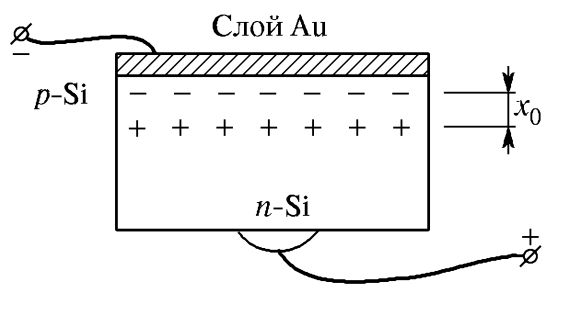
\includegraphics[width=0.45\textwidth]{images/detector.png}
		\caption{Схема полупроводникового детектора.}
		\label{img:detector}
	\end{figure}

	Рассмотрим принцип работы полупроводникового детектора (рис. \ref{img:detector}) \cite[с. 464-468]{labnik}. Детектор представляет собой обычно кремниевую пластинку из полупроводников n- и p-типа. В n-области находятся свободные электроны, в p-области находятся свободные дырки. Когда к пластинке прикладывается постоянное напряжение, как показано на рисунке, то свободные заряды покидают пластинку, в результате чего проводимость детектора уменьшается, при этом образуется обеднённая область шириной $x_0$. Альфа-частица энергией $E_i$ пролетает через обеднённую область детектора и ионизует атомы полупроводника переводя электроны из валентной зоны в свободную. В результате ионизации образуется пара электрон-дырка и возникает ток под действием приложенного к детектору напряжения. Этот ток усиливается зарядочувствительным усилителем, напряжение на котором пропорционально заряду, протекающему через усилитель. Напряжение на усилителе измеряется АЦП. Ток через усилитель пропорционален числу образованных пар электрон-дырка в детекторе. На образование одной такой пары в среднем расходуется энергия $E_{ср} = 3.6 \eV$. Предполагая, что альфа-частица расходует всю свою энергию $E_i$ на ионизацию атомов в обеднённом слое, можно оценить среднее количество образовавшихся пар электрон-дырка $N$:
	$$
	N_i = \frac{E_i}{E_{ср}}
	$$
	Предполагается, что ионизация атомов происходит независимо друг от друга с фиксированной интенсивностью, тогда количество ионизованных атомов подчиняется распределению Пуассона. Так как $N_i$ велико ($E_i \sim 1 \MeV$, $N_i \sim 10^5$), то распределение Пуассона приближается к распределению Гаусса с средним значением $N_i$ и среднеквадратичным отклонением $\sigma = \sqrt{N_i}$. \textit{Разрешающая способность детектора} определяется как отношение среднеквадратичного отклонения к среднему значению:
	$$
	R_{фл} = \frac{\sqrt{N_i}}{N_i} = \frac{1}{\sqrt{N_i}}
	$$
	
	Пусть в измеренной спектрограмме средняя энергия альфа-частиц составляет $E_i$, полуширина пика на половине высоты $\Delta E_i$, тогда \textit{энергетическая разрешающая способность} спектрометра равна:
	$$
	R = \frac{\Delta E_i}{E_i}
	$$
	Разрешающая способность спектрометра зависит от разрешающей способности детектора и от уровня шума в электронной схеме.
			
	% В приложении 1 приведены схемы последовательных радиоактивных распадов для исследуемых в работе элементов, составленные на основе информации из справочника \cite{manual}.
		
	\subsection*{Описание экспериментальной установки}
	
	Схема экспериментальной установки приведена на рисунке \ref{img:exp_scheme}:
		
	\begin{figure}[H]
		\centering
		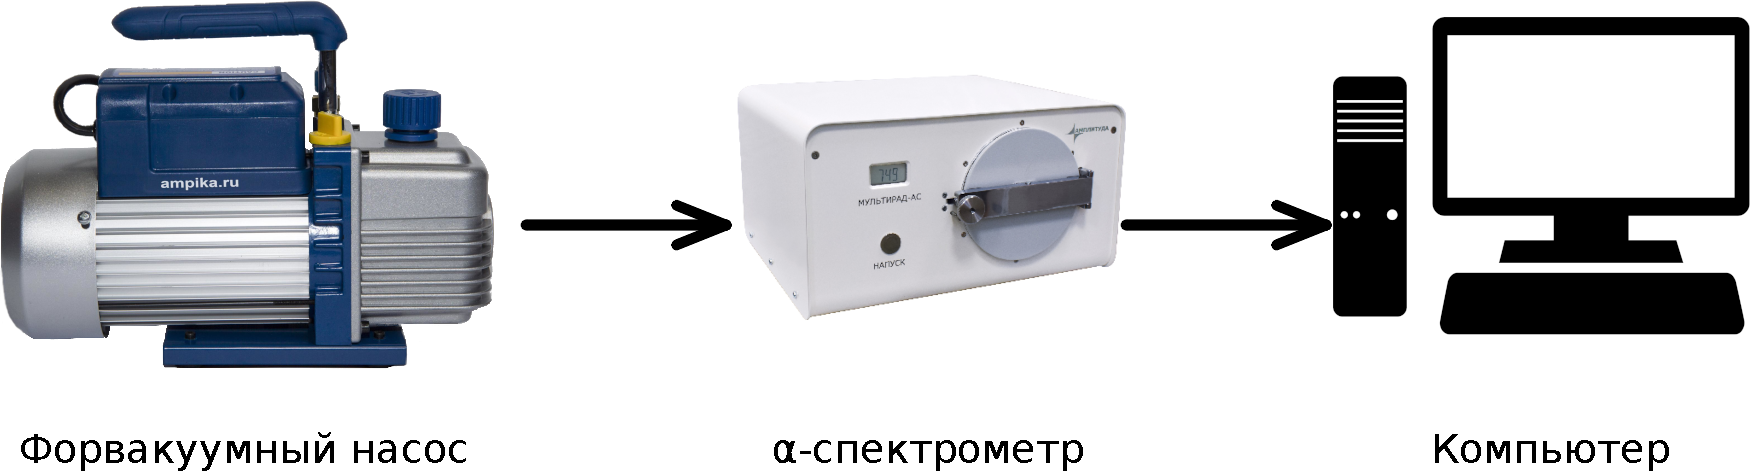
\includegraphics[width=1\textwidth]{images/exp_scheme.png}
		\caption{Схема экспериментальной установки.}
		\label{img:exp_scheme}
	\end{figure}

	Форвакуумный насос соединён с корпусом альфа-спектрометра вакуумным шлангом для откачки измерительной камеры до давлений $0.4 \div 20 \mmhg$. В камеру альфа-спектрометра на специальный столик помещается радиоактивный препарат. Над столиком находится полупроводниковый детектор частиц, который регистрирует альфа-частицы в диапазоне энергий $4.0 \div 9.5 \MeV$. Сигнал с детектора усиливается и подаётся на 12-битный АЦП. То есть спектрометр имеет 4096 каналов измерения энергий альфа-частиц. Результаты измерений передаются на компьютер, который проводит первичную обработку данных -- строит спектр радиоактивного распада. На подложку стола подаётся отрицательный относительно корпуса потенциал, чтобы ядра отдачи с импульсом направленным к детектору не попадали на него и не загрязняли его.
	
	\subsection*{Оборудование и приборы}
	\begin{enumerate}
		\item Форвакуумный насос Value VE-215N. Остаточное давление: $0.00002 \; \atm = 0.0152 \;\mmhg$.
		
		\item Альфа-спектрометр Амплитуда НТЦ Мультирад-АС. Диапазон энергии регистрируемого излучения $4.0 \div 9.5 \MeV$. Диапазон измерения активности $1 \cdot 10^2 \div 5 \cdot 10^5 \Bk$. Пределы допускаемой основной относительной погрешности измерений активности в исследуемых образцах $\varepsilon = 10 \%$. Максимальное значение входной нагрузки статистически распределённых импульсов не менее $10^4 \; \frac{имп}{с}$. Диапазон поддерживаемого в камере давления $0.4 \div 20.0 \mmhg$. Уровень собственного фона не более $100 \frac{имп}{сутки}$.
	\end{enumerate}
	
	\subsection*{Методика эксперимента}
	
	Так как зависимость энергии альфа-частицы от номера зарегистрировавшего её канала спектрометра не известна, то в начале работы проводится градуировка детектора. Для этого измеряется спектр излучения $\Ra$ в течение примерно 10 минут, каждому пику на графике спектра ставится в соответствие энергия зарегистрированной альфа-частицы. Так как амплитуда сигнала на выходе детектора пропорциональна энергии альфа-частицы, то градуировочная кривая должна быть прямой.
	
	После градуировки детектора измеряются спектры $\Po$, $\Pu$, $\Ua$ и смеси ($\Th$ и $\Am$) в течение примерно 10 минут. По градуировочной зависимости определяются энергии зарегистрированных альфа-частиц, и по справочнику определяются атомы, в результате радиоактивного распада которых образовалась альфа-частица.
	
	\subsection*{Обсуждение экспериментальных результатов}
	
	\subsubsection*{Градуировка детектора}
	По известным значениям энергии $\alpha$-частицы при распаде $\Ra$ и его дочерних ядер, определяются коэффициенты $a$ и $b$ градуировочной кривой детектора:
	$$
	E_i = a\cdot N_i + b.
	$$
	
	График градуировочной кривой $E_i(N_i)$ изображен на рисунке \ref{fig:w-channel}. С помощью метода наименьших квадратов были получены следующие градуировочные коэффициенты:
	
	$$ a = (2.97 \pm 0.01) \cdot 10^{-3} \; \frac{ \text{МэВ} }{ \text{кан.} },$$
	$$ b = (-0.10 \pm 0.02) \; \text{МэВ}.$$
	
	\begin{figure}[H]
		\includegraphics[width=1\textwidth]{gen/fig-w-channel.pdf}
		\caption{Зависимость энергии $\alpha$-частицы от номера канала $E_i(N_i)$.}
		\label{fig:w-channel}
	\end{figure}
	
	Согласно теории сдвиг по энергии $b$ должен быть равен 0. Систематическая ошибка, вносимая этим сдвигом $\varepsilon \sim 2\%$. Далее в таблицах будет приведена только случайная составляющая ошибок, чтобы иметь представление об их порядке. Полная погрешность оценивается по формуле:
	
	$$\varepsilon_\Sigma = \sqrt{\varepsilon^2 + \varepsilon_{E_i}^2}$$
	
	\subsubsection*{Исследование спектров $\alpha$-распада}
	
	С помощью градуировочной зависимости, определялась энергия альфа-частиц для всех остальных элементов: $\Ra$, $\Am + \Th$, $\Pu$, $\Ua$.
	
	В таблицах для каждой последовательности радиоактивных распадов приведены: $N_i$ -- средний номер канала, зарегистрировавший альфа-частицу с фиксированной энергией, $\Delta N_i$ -- среднеквадратичное отклонение в единицах каналов, $E_i$ -- средняя энергия зарегистрированных альфа-частиц, ширина $\Delta E_i$ -- среднеквадратичное отклонение в энергетических единицах, $\sigma_x$ -- случайная составляющая  ошибки определения величины $x$.
	
	Оценка погрешности проводилась по формуле погрешности косвенных измерений:
	$$ 
	\varepsilon_{R_{f,i}} = \frac{1}{2} \sqrt{\varepsilon_\Sigma^2 + \left(\frac{0.05}{3.60}\right)^2} \sim 1.5 \%
	$$
	$$ 
	\varepsilon_{R_i} = \sqrt{\varepsilon_{E_i}^2 + \varepsilon_{\Sigma}^2} \approx  \varepsilon_{\Sigma} \sim 2 \%
	$$
	
	\begin{figure}[H]
		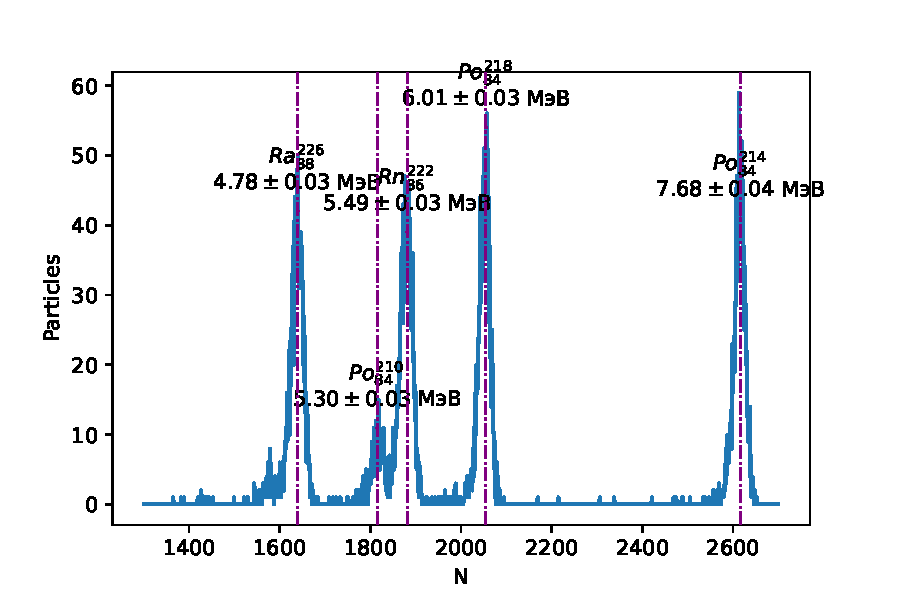
\includegraphics[width=1\textwidth]{gen/fig-ra.pdf}
		\caption{Спектр $\Ra$.}
		\label{fig:ra}
	\end{figure}

	\vspace*{-1cm}
	
	\begin{table}[H]
		\addtolength{\tabcolsep}{-4pt}
		\footnotesize
		\begin{tabular}{cccccc}
\toprule
$N_i$ & $dN_i$ & $E_i$, МэВ & $\sigma_{E_i}$, МэВ & $\Delta E_i$, МэВ & $\sigma_{\Delta E_i}$, МэВ \\
\midrule
1640.0 & 24.33 & 4.78 & 0.03 & 0.0723 & 0.0003 \\
1815.0 & 22.58 & 5.30 & 0.03 & 0.0671 & 0.0002 \\
1881.0 & 23.97 & 5.49 & 0.03 & 0.0712 & 0.0003 \\
2055.0 & 21.05 & 6.01 & 0.03 & 0.0626 & 0.0002 \\
2617.0 & 22.50 & 7.68 & 0.04 & 0.0669 & 0.0002 \\
\bottomrule
\end{tabular}

		\caption{Энергии пиков $\Ra$.}
		\label{tab:term}
	\end{table}
	
	\vspace*{-1cm}
	
	\begin{figure}[H]
		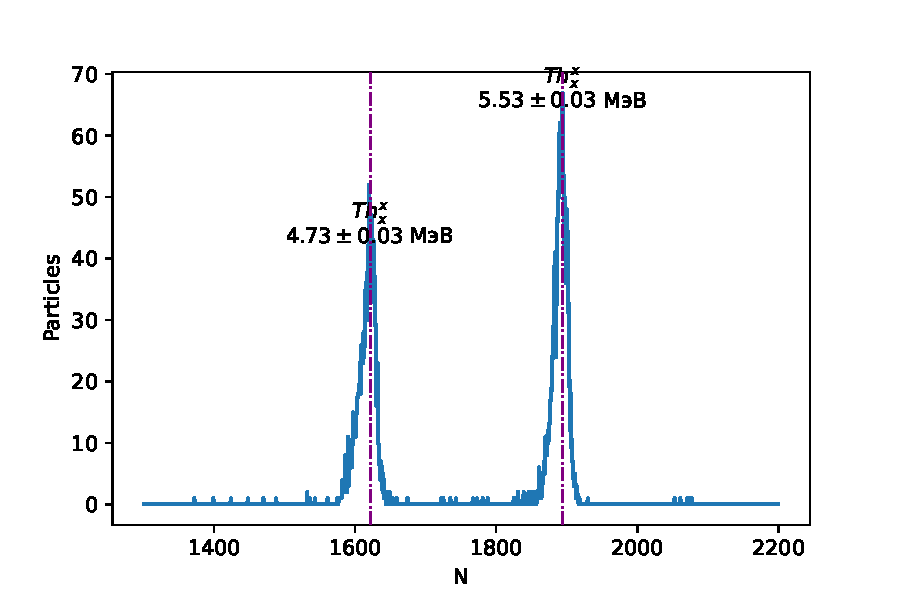
\includegraphics[width=1\textwidth]{gen/fig-th_am.pdf}
		\caption{Спектр $\Am + \Th$.}
		\label{fig:th_am}
	\end{figure}
	
	\vspace*{-1cm}
	
	\begin{table}[H]
		\addtolength{\tabcolsep}{-4pt}
		\footnotesize
		\begin{tabular}{ccccccc}
\toprule
$N_i$ & $\Delta N_i$ & $E_i$, МэВ & $\varepsilon_{E_i}, \%$ & $\Delta E_i$, МэВ & $R_i \cdot 10^2$ & $R_{f,i} \cdot 10^2$ \\
\midrule
1622 & 15.80 & 4.73 & 0.6 & 0.0469 & 0.99 & 0.087 \\
1894 & 17.12 & 5.53 & 0.6 & 0.0509 & 0.92 & 0.081 \\
\bottomrule
\end{tabular}

		\caption{Энергии пиков $\Am + \Th$.}
		\label{tab:th_am}
	\end{table}
	
	\vspace*{-1cm}
	
	\begin{figure}[H]
		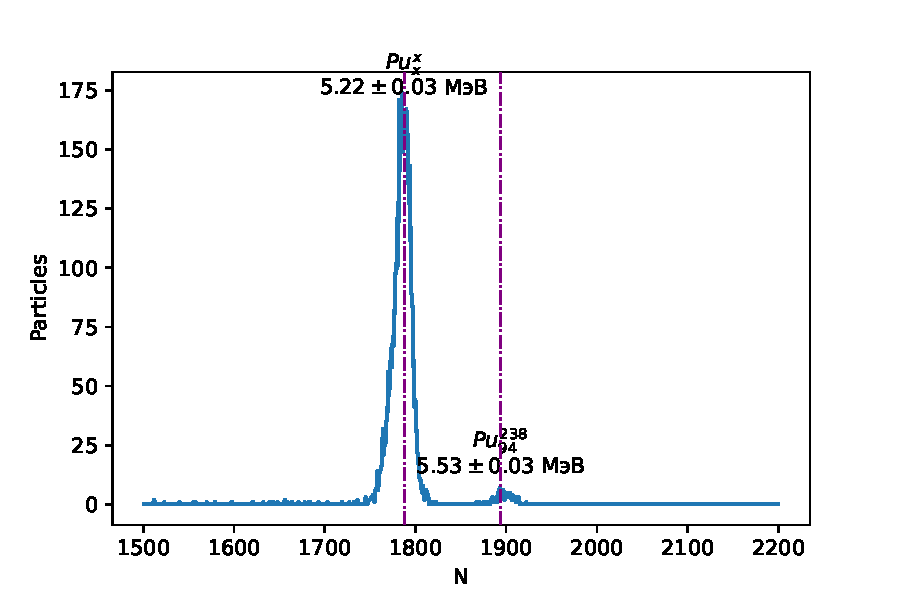
\includegraphics[width=1\textwidth]{gen/fig-pu.pdf}
		\caption{Спектр $\Pu$.}
		\label{fig:pu}
	\end{figure}
	
	\vspace*{-1cm}
	
	\begin{table}[H]
		\addtolength{\tabcolsep}{-4pt}
		\footnotesize
		\begin{tabular}{ccccccc}
\toprule
$N_i$ & $\Delta N_i$ & $E_i$, МэВ & $\varepsilon_{E_i}, \%$ & $\Delta E_i$, МэВ & $R_i \cdot 10^2$ & $R_{f,i} \cdot 10^2$ \\
\midrule
1788 & 16.81 & 5.22 & 0.6 & 0.0500 & 0.96 & 0.083 \\
1894 & 20.90 & 5.53 & 0.6 & 0.0621 & 1.12 & 0.081 \\
\bottomrule
\end{tabular}

		\caption{Энергии пиков $\Pu$.}
		\label{tab:pu}
	\end{table}
	
	\vspace*{-1cm}
	
	\begin{figure}[H]
		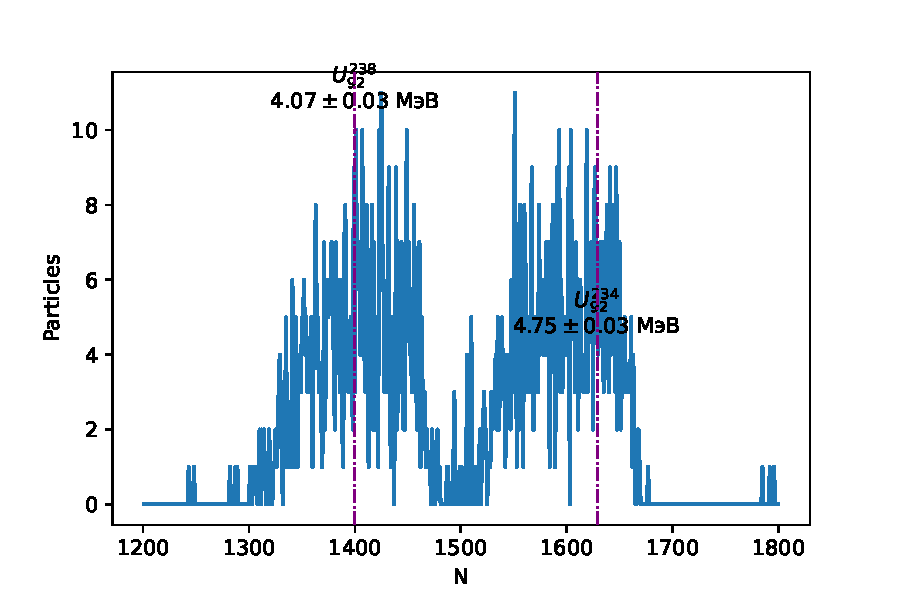
\includegraphics[width=1\textwidth]{gen/fig-u.pdf}
		\caption{Спектр $\Ua$.}
		\label{fig:u}
	\end{figure}
	
	\vspace*{-1cm}
	
	\begin{table}[H]
		\addtolength{\tabcolsep}{-4pt}
		\footnotesize
		\begin{tabular}{ccccccc}
\toprule
$N_i$ & $\Delta N_i$ & $E_i$, МэВ & $\varepsilon_{E_i}, \%$ & $\Delta E_i$, МэВ & $R_i \cdot 10^2$ & $R_{f,i} \cdot 10^2$ \\
\midrule
1400 & 87.96 & 4.07 & 0.7 & 0.2614 & 6.43 & 0.094 \\
1629 & 43.20 & 4.75 & 0.6 & 0.1284 & 2.71 & 0.087 \\
\bottomrule
\end{tabular}

		\caption{Энергии пиков $\Ua$.}
		\label{tab:u}
	\end{table}
	
	\subsubsection*{Проверка закона Гейгера-Нэттола}
		
	Зная энергии $\alpha$-распада $\text{Ra}_{88}^{226}$ и его дочерних ядер, а также периоды их полураспада, можно судить о точности выполнения закона Гейгера-Неттола. С этой целью проведем линеаризацию зависимости:
	
	\begin{figure}[H]
		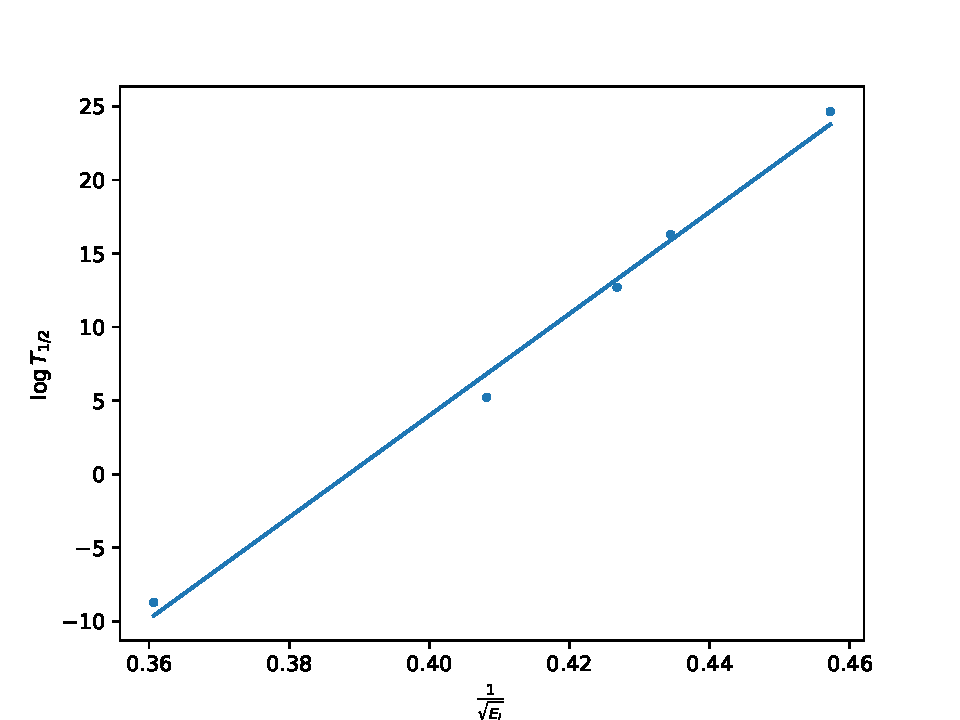
\includegraphics[width=1\textwidth]{gen/fig-te.pdf}
		\caption{График $\log{T_{1/2}} \left( \frac{1}{\sqrt{E_i}}\right)$.}
		\label{fig:te}
	\end{figure}

	Полученный график изображен на рисунке \ref{fig:te}. Коэффициент корреляции слабо отличается от единицы: 
	$$ \rho = \frac{ \text{cov}_{ xy } }{ \sigma_x \cdot \sigma_y} = 0.9964. $$
	
	\subsection*{Выводы}
	
	В работе были получены спектры $\alpha$-излучения ядер. Мы экспериментально определили энергетическое разрешение детектора (см. таблицы):
	
	$$R_i = \frac{\Delta E_i}{E_i},\; \varepsilon_{R_i} \sim 2 \%$$
	
	Оценка влияния статистической флуктуации числа электрон-дырочных пар $R_{f,i} = \sqrt{\frac{E_{\text{ср}}}{E_i}}, \; \varepsilon_{R_{f,i}} \sim 1.5 \%$, создаваемых падающей частицей, получилась на порядки меньше вычисленных энергетических разрешений $R_i$. Поэтому можно сделать вывод, что основной причиной разброса импульсов по амплитуде является шум электрических цепей.
	
	Был проверен закон Гейгера-Нэттола методом линеаризации зависимости. Коэффициент корреляции слабо отличается от единицы: 
	
	$$ \rho (x,y) = 0.9964. $$
	
	\begin{thebibliography}{}
		\bibitem{labnik} \textbf{Ципенюк, Ю.М.} Лабораторный практикум по общей физике. Квантовая физика: Учеб. пособие для вузов./ Ф.Ф.~Игошин, Ю.А.~Самарский, Ю.М.~Ципенюк; под. ред. Ю.М.~Ципенюка --- М.: Физматкнига, 2012. --- 464 с. ISBN 978-5-89155-206-7.
		
		\bibitem{Sivukhin5} \textbf{Сивухин, Д.В.} Общий курс физики: Учеб. пособие: Для вузов. В 5 т. Т.V. Атомная и ядерная физика. --- 3-е изд., стереот. --- М.: ФИЗМАТЛИТ, 2020. --- 784 с. ISBN 978-5-9221-0645-0 (Т. V).
		
		\begin{comment}
		\bibitem{manual} \textbf{Голашвили, Т.В.} Справочник нуклидов./ Т.В.~Голашвили, В.П.~Чечев, С.А.~Бадиков; под. ред. Т.В.~Голашвили. --- 4-е изд., перераб. и доп. --- М.: Издательский дом МЭИ, 2011. --- 462 с. ISBN 978-5-383-00513-2. 
		\end{comment}
	\end{thebibliography}
	
	\begin{comment}
	\newpage

	\subsection*{Приложение 1. Схемы последовательных радиоактивных распадов}
	
	Приведём схемы последовательных радиоактивных распадов для исследуемых в работе элементов, составленные на основе информации из справочника \cite{manual}. Над стрелочкой указан тип радиоактивного распада: $\alpha$ -- альфа-распад, $\beta^-$ -- бета-распад с испусканием электрона. Под стрелочкой в первой строке указывается полупериод распада. Если известна энергия излучения, то она указывается во второй строке. В случае, если возможно несколько вариантов радиоактивного распада, то в третьей указывается вероятность распада в \%. Условные обозначения для периода полураспада: $\msec[]$ -- миллисекунды, $\sec[]$ -- секунды, $\min[]$ -- минуты, $\hour[]$ -- часы, $\day[]$ -- дни, $\year[]$ -- года. Если для энергии излучения не указаны единицы измерения, то энергия измеряется в $\MeV[]$. Если известна погрешность, то она указывается в круглых скобках в единицах младшего значащего разряда. Например, $45.1(32)$ означает $45.1 \pm 3.2$. Обозначение $\stable[]$ означает, что атом является стабильным и цепочка радиоактивных распадов заканчивается.
	
	\subsubsection*{Последовательность радиоактивных распадов $\Ra$}
	
	$\Ra \adecay{1600(7) \year}{4.773(3)} \elem{Rn}{222}{86} \adecay{3.8235(4) \day}{5.490} \elem{Po}{218}{84}$ \\
	%
	$\elem{Po}{218}{84} \avdecay{3.10(2) \min}{6.000}{99.98(2) \%} \elem{Pb}{214}{82} \bmdecay{26.8(9) \min}{0.218(5)} \elem{Bi}{214}{83}$ \\
	%
	$\elem{Po}{218}{84} \bmvdecay{3.10(2) \min}{}{0.02(2) \%} \elem{At}{218}{85}$ \\
	%
	%
	$\elem{At}{218}{85} \avdecay{1.5(3) \sec}{6.690}{99.9 \%} \elem{Bi}{214}{83}$ \\
	%
	$\elem{At}{218}{85} \bmvdecay{1.5(3) \sec}{}{0.1 \%} \elem{Rn}{218}{86}$ \\
	%
	$\elem{Rn}{218}{86} \adecay{35(5) \msec}{7.130} \elem{Pb}{214}{82} \bmdecay{26.8(9) \min}{0.218(5)} \elem{Bi}{214}{83}$ \\
	%
	%
	$\elem{Bi}{214}{83} \avdecay{19.9(4) \min}{1.4 \keV}{0.021(1) \%} \elem{Tl}{210}{81} \bmdecay{1.30(3) \min}{1.184(14)} \elem{Pb}{210}{82}$ \\
	%
	$\elem{Bi}{214}{83} \bmvdecay{19.9(4) \min}{0.642(6)}{99.979(1) \%} \elem{Po}{214}{84} \adecay{1.643(20) \cdot 10^{-6} \sec}{7.6867(1)} \elem{Pb}{210}{82}$ \\
	%
	%
	$\elem{Pb}{210}{82} \avdecay{22.2(2) \year}{}{1.9(7) \cdot 10^{-6} \%} \elem{Hg}{206}{80} \bmdecay{8.15(10) \min}{0.392(5)} \elem{Tl}{206}{81}$ \\
	%
	$\elem{Pb}{210}{82} \bmvdecay{22.2(2) \year}{6.08(17) \keV}{\approx 100 \%} \elem{Bi}{210}{83}$ \\
	%
	%
	$\elem{Bi}{210}{83} \avdecay{5.013(5) \day}{}{1.3 \cdot 10^{-4} \%} \elem{Tl}{206}{81}$
	%
	$\elem{Bi}{210}{83} \bmvdecay{5.013(5) \day}{0.39}{\approx 100 \%} \elem{Po}{210}{84}$	
	%
	%
	$\elem{Po}{210}{84} \adecay{138.376(2) \day}{5.3} \elem{Pb}{206}{82} \stable$ \\
	%
	$\elem{Tl}{206}{81} \bmdecay{4.2(17) \min}{0.538(3)} \elem{Pb}{206}{82} \stable$ \\
	%
	
	\subsubsection*{Последовательность радиоактивных распадов $\Pu$}
	
	$\Pu \adecay{24110(30) \year}{5.1} \elem{U}{235}{92} \adecay{7.04(1)\cdot10^8 \year}{4.378(5)} \elem{Th}{231}{90}$ \\
	%
	$\elem{Th}{231}{90} \bmdecay{25.52(1) \hour}{77.1(13) \keV} \elem{Pa}{231}{91} \adecay{3.276(110 \cdot 10^4 \year)}{4.92} \elem{Ac}{227}{89}$ \\
	%
	%
	$\elem{Ac}{227}{89} \bmvdecay{21.772(3) \year}{10 \keV}{98.62(36) \%} \elem{Th}{227}{90} \adecay{18.68(9) \year}{5.9} \elem{Ra}{223}{88}$ \\
	%
	$\elem{Ac}{227}{89} \avdecay{21.772(3) \year}{67 \keV}{1.38(36) \%} \elem{Fr}{223}{87}$ \\
	%
	$\elem{Ra}{223}{88} \adecay{11.43(5) \day}{5.7} \elem{Rn}{219}{86}$
	%
		
	%\item $\Pu$:
		
	%\item $\Po$:
		
	%\item $\Ua$:
		
	%\item Смесь $\Th$ и $\Am$:
	
	\end{comment}
		
\end{multicols}
\end{document}